\documentclass[english,twoside, openright]{report}
\usepackage[utf8]{inputenc}
\usepackage{babel}
\usepackage{physics}
\usepackage{xcolor}
\usepackage{amsmath}
\usepackage{amsfonts}
\usepackage{lineno,hyperref}
\usepackage{hyperref}

\usepackage{tikz}
\usetikzlibrary{arrows, decorations.markings}

\tikzstyle{vecArrow} = [thick, decoration={markings,mark=at position
   1 with {\arrow[semithick]{open triangle 60}}},
   double distance=1.4pt, shorten >= 5.5pt,
   preaction = {decorate},
   postaction = {draw,line width=1.4pt, white,shorten >= 4.5pt}]
\tikzstyle{innerWhite} = [semithick, white,line width=1.4pt, shorten >= 4.5pt]

\newcommand{\cas}[2]{
  \mathcal{C}_{#1}\left[#2\right]
  }

\author{Jamil KR}
\title{$U_p(4)\; \times\; U_q(4)$}
\begin{document}
\maketitle

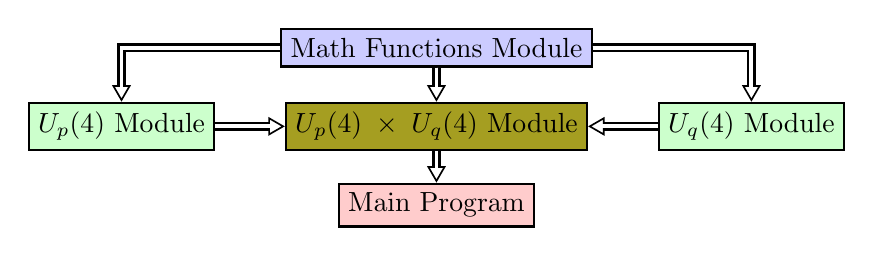
\begin{tikzpicture}[thick]
  \node[draw,rectangle,fill=green!20] at (-3,0)(a){$U_p(4)$ Module};
  \node[draw,rectangle,fill=olive!80,right of=a] at (0,0)(c){$U_p(4)\;\times\;U_q(4)$ Module};
  \node[draw,rectangle,fill=green!20,right of=c]at(4,0)(b){$U_q(4)$ Module};
  \node[draw,rectangle,fill=blue!20,above of=c](d){Math Functions Module};
  \node[draw,rectangle,fill=red!20,below of=c](e){Main Program};
  
  \draw[vecArrow] (a) to (c);
  \draw[vecArrow] (b) to (c);
  \draw[vecArrow] (d) to (c);
  \draw[vecArrow] (c) to (e);
  \draw[vecArrow] (d) -| (a);
  \draw[vecArrow] (d) -| (b);

  \draw[innerWhite] (a) to (c);
  \draw[innerWhite] (b) to (c);
  \draw[innerWhite] (d) to (c);
  \draw[innerWhite] (c) to (e);
  \draw[innerWhite] (d) -| (a);
  \draw[innerWhite] (d) -| (b);
\end{tikzpicture}

\section{Math Functions Module $\rightarrow$ \texttt{MOD\_matfun.f90}}

\begin{itemize}
\item Functions:
  \begin{itemize}
  \item \texttt{p\_symbol}(a,b) $=\; (a)_s\;=\;a(a+1)...(a+s-1)$
  \end{itemize}
\end{itemize}

\section{$U_p(4)$ Module $\rightarrow$ \texttt{MOD\_Up4.f90}}
Hamiltonian:

\begin{equation}
  \hat{H}_{U_p(4)} = \beta \; \cas{2}{so_p(4)} + \gamma \; \cas{2}{so_p(3)} + \gamma_2 \; \left[\cas{2}{so_p(3)}\right]^2 + \kappa \; \cas{2}{so_p(4)}\cas{2}{so_p(3)}
\end{equation}

\begin{itemize}
\item Global definitions:
  \begin{itemize}
  \item Npval: $U(4)$ Totally symmetric representation.
  \end{itemize}
\item Functions:
  \begin{itemize}
  \item Function: \texttt{RME\_Casimir\_SOp4}
  \item Function: \texttt{RME\_Casimir\_SOp3}
  \item Function: \texttt{RME\_Qp2}
  \end{itemize}
\end{itemize}

\section{$U_q(4)$ Module $\rightarrow$ \texttt{MOD\_Uq4.f90}}

Hamiltonian:

\begin{equation}
  \hat{H}_{U_q(4)} = a \; \cas{1}{u_q(3)} + b \; \cas{2}{u_q(3)} + c \; \cas{2}{so_q(3)} + d \; \cas{2}{so_q(4)}
\end{equation}

\begin{itemize}
\item Global definitions:
  \begin{itemize}
  \item Nqval: $U(4)$ Totally symmetric representation.
  \end{itemize}
\item Functions:
  \begin{itemize}
  \item Function: \texttt{RME\_Casimir\_Uq3}
  \item Function: \texttt{RME\_Casimir\_SOq3}
  \item Function: \texttt{RME\_Casimir\_SOq4}
  \item Function: \texttt{RME\_Qq2}
  \end{itemize}
\end{itemize}

\section{$U_p(4)\;\times\;U_q(4)$ Module $\rightarrow$ \texttt{MOD\_Up\_x\_Uq.f90}}

\end{document}